\documentclass{article}

\usepackage{graphicx}
\usepackage{gensymb}

\title{Numerical Calculation of the Space Shuttle's Ascent Trajectory}
\author{Micaiah Smith-Pierce}
\date{\it{22-April-2017}}

\begin{document}
\maketitle

\section{Abstract}

In this assignment, an iterative numerical process was used to calculate the trajectory of the Space Shuttle during ascent.
The trajectory was computed
by repeatedly incrimenting a time step and using basic physical models to calculate a new state from the old state. Design parameters
such as mass, fuel capacity, and thrust were found online and used to inform the calculations. Based on the required orbit altitude, some variables
that can be controlled during the ascent were manipulated until a stable orbit after main engine cut off was obtained. The calculated trajectory
was compared to the actual trajectory. The results were reasonably similar to the actual shuttle's performance.

\section{Nomenclature}
\begin{tabular}{l l}
A & maximum (forward-facing) cross-sectional area \\
$a_r$ & radial acceleration \\
$a_\theta$ & tangential acceleration \\
$C_d$ & drag coefficient with respect to A \\
d & drag force \\
g & the acceleration due to gravity \it at the current altitude \it \\
$g_0$ & the acceleration due to gravity at sea level \\
h & altitude \\
$I_{sp}$ & specific impulse \\
m & gross mass of the system \\
max q & the maximum value of q experienced during the ascent \\
MECO & the point in time at which the Main Engines Cut Off \\
q & dynamic pressure \\
$R_e$ & radius of the earth \\
$\rho$ & air density \\
SRB & Solid Rocket Booster \\
stage 1 & the period before the SRBs separate \\
stage 2 & the period in between SRB separation and MECO \\
T & total thrust \\
t+ & indicates that the following number is the number of seconds after liftoff (e.g. t+60)\\
$\theta_{pitch}$ & pitch angle \\
$v_r$ & radial (upward) velocity \\
$v_\theta$ & tangential velocity in an inertial reference frame (i.e. starts at rotational speed of the earth)\\
\end{tabular}


Note: Dot notation is used to represent the derivative with respect to time, e.g. $\dot{x} = \frac{\partial x}{\partial t}$.

\section{Introduction}

It is customary for AE 1601 classes to do an assignment involving flight dynamics of rockets. Rather than assign the standard project which
involves building a model rocket, Professor Komerath has assigned his students a much more theoretical and computation-intensive assignment
which promotes and requires a thorough understanding of rocket mechanics. He has required his students to compute the trajectory during the
ascent phase of a mission of NASA's space shuttle.

The Space Shuttle is a spacecraft which is intended to launch an orbiter with research payload into orbit. It consists of an orbiter with
3 cryogenic main engines, an external tank which carries LO2 and LH2 fuel for th main engines and two SRBs. The ascent phase proceeds as follows:
For the first stage, the SRBs provide the majority of the thrust. Then, as soon as the SRBs run out of fuel, they are jettisoned to reduce the mass
of the system. Thus begins the second stage, where all of the thrust is provided by the three main engines. When the last of the liquid fuel
has been burned, the orbiter has been injected into a circular orbit, the main engines cut out, and the external tank is jetisoned.

There are two additional considerations. First, the max q must not exceed 27 kPa. Also, the acceleration must remain below $3g_0$. If
either of these constraints are violated, the structure may fail and the astronauts may be injured.

\section{Theoretical Analysis}

The most notable force on the rocket is due to thrust (the force due to gravity is not treated in this section. Rather than consider a force
due to gravity, the acceleration due to gravity is simply added to the rocket's acceleration. See below). The thrust and $I_{sp}$ are a function
of the air density. However, the manner in which they vary are beyond my understanding, so I assumed that both the thrust and $I_{sp}$ vary
linearly with $\rho$. I used linear interpolation based on $\rho$ between the value at vacuum and the value at sea level in order to estimate
the values at a given altitude.

q and drag were calculated using the standard equations
\[q = \frac{1}{2}\rho v^2\]
\[d = C_d*q*A\]
$C_d$ was chosen as 0.5. This is higher than the value which Prof. Komerath recommended. However, the drag coefficient of the Saturn V rocket
was approximately 0.5, according to some admittedly dubious sources \cite{forum}, and as the space shuttle is more geometrically complex than
the Saturn V, its $C_d$ should be at least as high. In any case, some different drag values were tested, and they made little difference as to
the final trajectory.

The acceleration due to the thrust and drag forces was computed by dividing the total force by the mass of the rocket, which was computed at every
time step using the fuel loss rate. The mass of fuel lost can be computed as
\[\dot{m} = \frac{T}{I_{sp} g_0}\].
Of course, the solid fuel loss and liquid fuel loss had to be treated separately, and the mass of the boosters had to be subtracted at separation.

The acceleration in the radial and tangential directions were calculated using the forces, and a number of other terms. The acceleration due to
gravity was calculated at each altitude, as well as the centrifugal and coriolis accelerations. All of these were taken into account and added
to the thrust and drag acceleration. The equations are:

\[a_r = \frac{T - d}{m} sin(\theta_{pitch}) - g + \frac{v_\theta^2}{R_e + h}\]
\[a_\theta = \frac{T - d}{m} cos(\theta_{pitch}) - \frac{v_r v_\theta}{R_e + h}\]

The rotation of the earth was taken into account when initializing the horizontal velocity. Thus, the trajectory represented injection into
an equatorial and not a polar orbit.

\section{Computations}

The trajectory was computed using an iterative algorithm in MATLAB. The mass, altitude, horizontal and vertical speed, time, and
angular displacement were initialized, and then repeatedly incrimented using a time step of 0.1 second. q and g were computed directly
at each time. $\rho$ was estimated using linear interpolation between datapoints on a standard atmosphere table taken from \cite{atmo} (and
assumed to be zero for altitudes above the last data point).

The thrust and pitch are unique in that they can be controlled arbitrarily. The thrust was set to its maximum possible value at most stages
during the ascent. However, it was decreased from t+ 26 to t+ 60 seconds, as it was for the real shuttle \cite{ksc}, in order to control max q,
and decreased again in the second stage by exactly the amount necessary to keep the acceleration below 3g. The pitch, on the other hand,
was calibrated via a painstaking trial-and-error process until the shuttle was injected into a stable orbit at the highest possible altitude.
The fact that in the first 20 seconds it should go from $90\degree$ to $83\degree$ was taken from \cite{ksc}. After that, it was set by trial
and error. If it is set too low too early, the orbit altitude will decrease, but if it remains too high too late, the shuttle will not have
sufficient tangential velocity in order to maintain a stable orbit.

Engine data for the solid rocket boosters was taken primarily from \cite{srb} and data on the cryogenic engiens was taken from \cite{rs}.

\section{Results}

The physical models correctly predicted the trajectory of the shuttle based on the inputs. However, it turned out to be extremely important
that the pitch control be chosen judiciously. In Figure \ref{eccentric} below, nothing has been changed from a realistic mission except
that the pitch was allowed to remain at $83 \degree$ for the majority of the flight, rather than be decreased at high altitude. Obviously,
this orbit is unacceptable because shuttle would collide with the earth. This trial
also serves to confirm that the orbital mechanics were correctly implimented. Up to a visual inspection, the trajectory is an elipse with
the center of the earth at one focus, as Kepler's laws require.

When the pitch was appropriately controlled, the shuttle reached a stable orbit at an altitude of 155 km. This is noticeably lower than the
actual orbit altitude of the real shuttle, which is at least 186 km \cite{ksc}. You may notice that the altitude v. time plot is a bit
"lumpy", which is because the pitch values at every time were determined by trial and error and varied in discrete steps (i.e., I am a bad
pilot). Max q was 27 kPa as intended
and occurred shortly after t+ 60 seconds as expected. boosters separate at an altitude of 40 km, rather than 50 km \cite{ksc}. MECO occurred
at 536 seconds, which is comparable to what happened in real life. More detailed results are plotted below. Note that the main engine thrust
is not constant with time. In the first stage, it increases due to the increasing density, except for the interval where it is artificially
decreased to minimize max q. It is constant for a period after the shuttle leaves the atmosphere, and then begins to drop off in the period
where it is decreased in order to keep the acceleration below 3g. See figures below for plots of altitude, trajectory, q, and thrust data.


\begin{figure}
	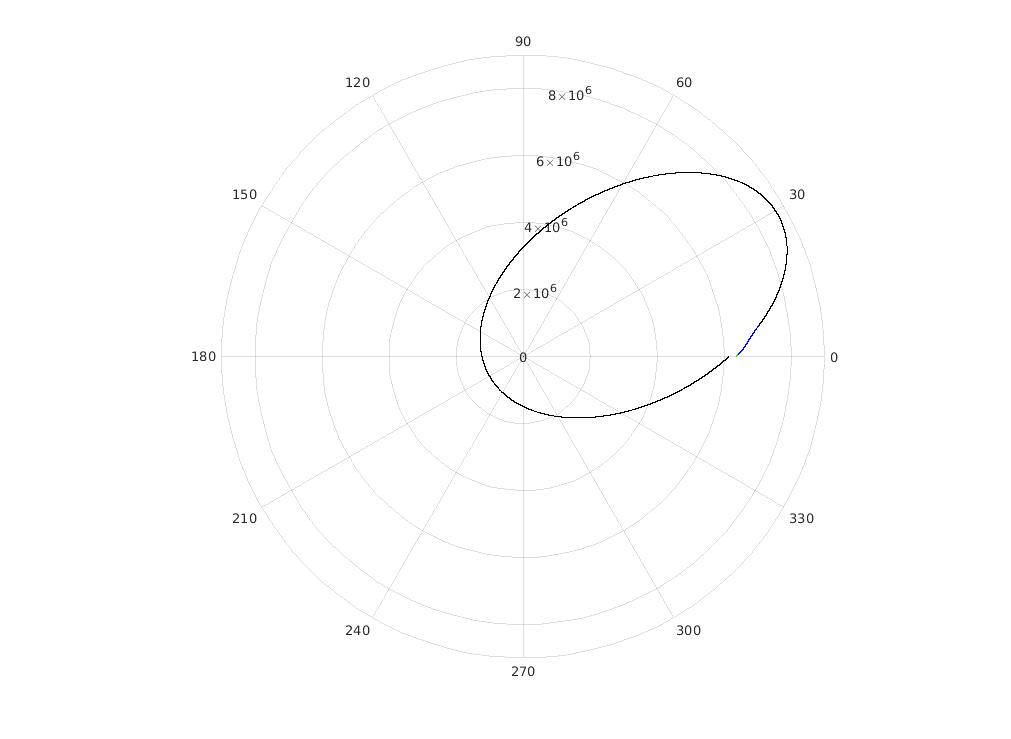
\includegraphics[width = \linewidth]{space_shuttle_to_steep.jpg}
	\caption{The orbit of the space shuttle when the pitch is inappropriately calibrated}
	\label{eccentric}
\end{figure}


\begin{figure}
	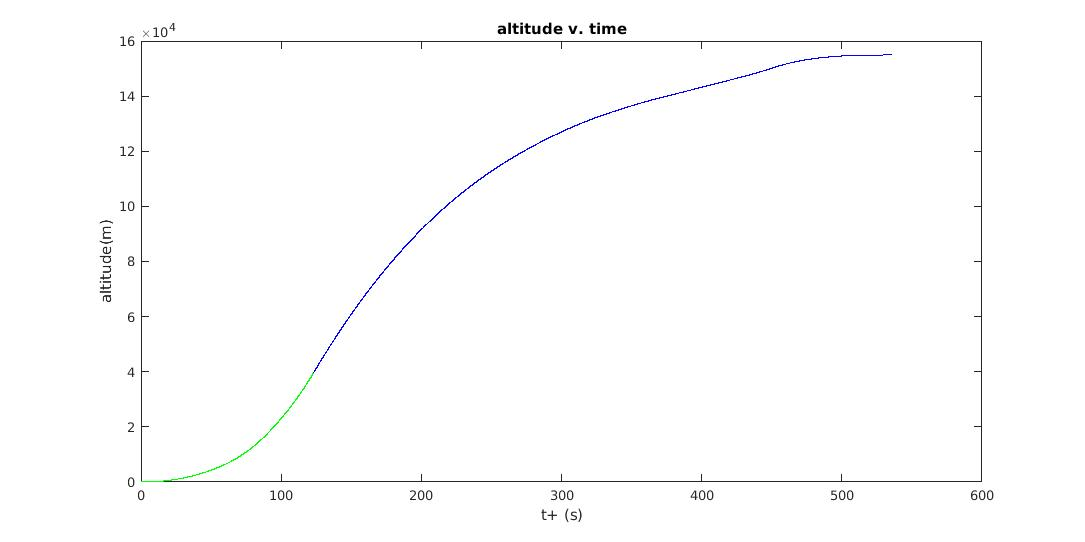
\includegraphics[width = \linewidth]{altitude_v_time.jpg}
	\caption{The altitude of the space shuttle plotted vs. time during ascent. The green line represents the first stage,
and the blue line represents the second stage.}
	\label{altitude}
\end{figure}
\begin{figure}
	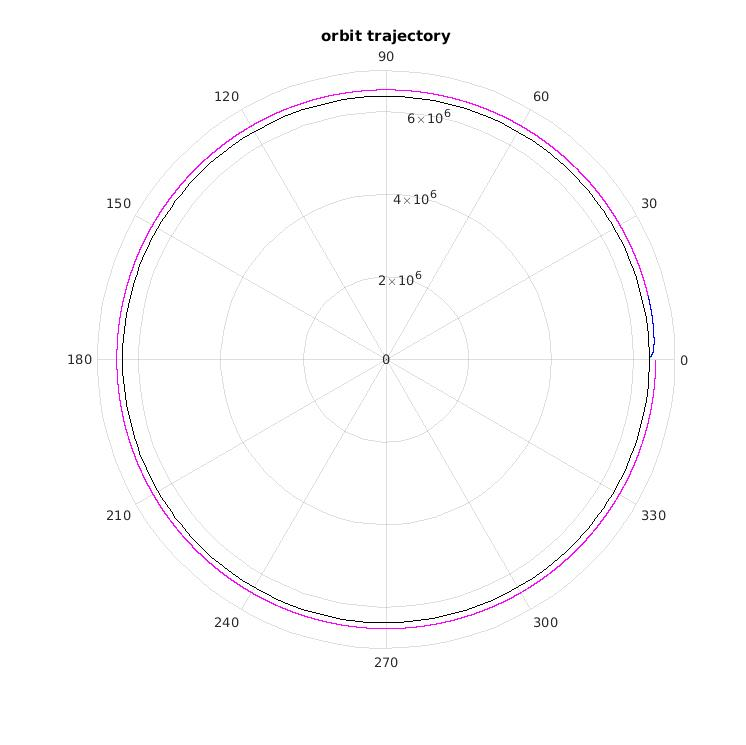
\includegraphics[width = \linewidth]{orbit_trajectory.jpg}
	\caption{The trajectory of the space shuttle. The green line represents the first stage,
the blue line represents the second stage, the magenta line represents orbit, and the black line represents the surface of the earth.}
	\label{trajectory}
\end{figure}
\begin{figure}
	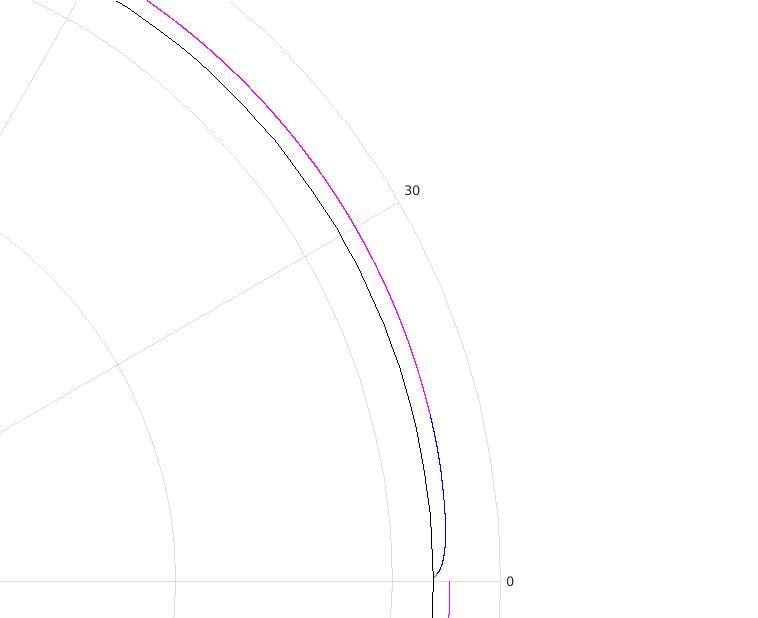
\includegraphics[width = \linewidth]{orbit_trajectory_zoom.jpg}
	\caption{The same plot as Figure \ref{trajectory}, except zoomed in for clarity}
	\label{zoom}
\end{figure}
\begin{figure}
	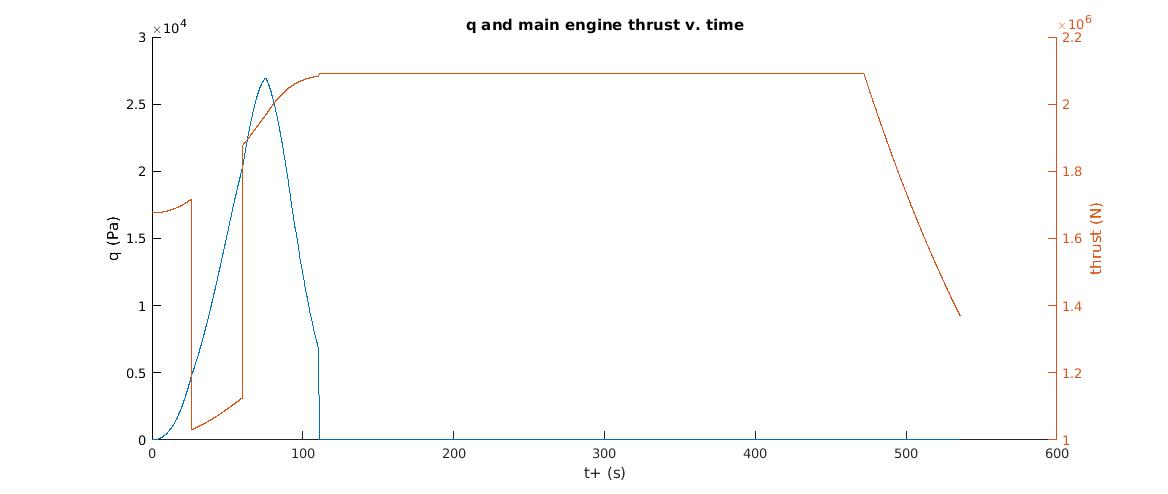
\includegraphics[width = \linewidth]{q_thrust.jpg}
	\caption{The dynamic pressure, and the combined thrust of all three RS-25 engines}
	\label{q_thrust}
\end{figure}


\section{Discussion}

Overall, the simulation was successful. It reproduced qualitatively all the phenomena observed in the real shuttle, and quantitatively it
was accurate well within a factor of two. However, judging from the booster separation altitude and the MECO altitude, the simulated shuttle
simply was generally inferior to the actual shuttle. This is intriguing, because generally idealized models have a tendency to overestimate
performance. A few possible reasons for the inaccuracy suggest themselves. First, the drag coefficient was little better than a guess.
However, varying the drag coefficient dramatically seemed to have only a small effect on the final results, so this is probably not the
problem. Also, the assumption that the thrust varies linearly with density could be less accurate than hoped. So, it is possible that
the thrust should have been higher than the values used in the simulation.

Alternatively, there is the fact that the real space shuttle had
professional orbital engineers planning its trajectory, whereas the simulation was conducted by an undergraduate student. While choosing
the pitch values, it became clear that choosing them inappropriately could dramatically reduce the shuttle's performance (consider what would
happen if the pitch was set to $0\degree$ at liftoff). It is entirely possible that by changing the pitch values the shuttle's performance
could be significantly improved. Finally, I have encountered refercences to orbital maneuvering systems on the orbiter itself, implying that it
may not have to be in a level, stable orbit at MECO. This could also potentially increase the orbit altitude which can be obtained.
In any case, it would be interesting to revisit this problem when my education has provided me with a more complete
knowledge of rocket engines and orbital mechanics to see if I can resolve the discrepancies between my calculations and empirical results.

\pagebreak
\begin{thebibliography}{5}
\bibitem{srb}
	Mark Wade
	\\\texttt{www.astronautix.com/s/srb.html}
\bibitem{rs}
	Aerojet Rocketdyne
	\\\texttt{http://www.rocket.com/rs-25-engine}
\bibitem{atmo}
	Engineering Toolbox
	\\\texttt{https://www.engineeringtoolbox.com/international-standard-atmosphere-d\_985.html}
\bibitem{ksc}
	Jim Dumoulin
	NASA Kenedy Space Center
	\\\texttt{https://science.ksc.nasa.gov/shuttle/technology/sts-newsref/mission\_profile.html}
\bibitem{forum}
	Space Stack Exchange
	\\\texttt{https://space.stackexchange.com/questions/12649/how-can-i-estimate-the-
coefficient-of-drag-on-a-saturn-v-rocket-a-simulator-or?utm\_medium=organic\&utm\_source
=google\_rich\_qa\&utm\_campaign=google\_rich\_qa}
\end{thebibliography}

\end{document}
